% Created 2026-06-17
% TikZ/MSC figures for etcd case study
% Figures:
%   1. etcd write path via Raft (MSC)
%   2. Lease lifecycle (TikZ timeline)
%   3. etcd cluster topology (TikZ)
\documentclass[tikz]{standalone}

\input{../../templates/tikzFigureHeader}
\usetikzlibrary{arrows.meta, positioning, backgrounds, shapes.geometric}

% Local aliases matching consistency_mscs.tex convention
\newcommand{\mscwrite}[2]{\found{}{#1}{#2}}
\newcommand{\mscread}[2]{\lost[side=right]{}{#1}{#2}}

\begin{document}

% ============================================================
% Figure 1: etcd linearizable write via Raft
%
% Shows: client put → leader AppendEntries to both followers →
%        quorum ACK (F1 alone sufficient for 3-node cluster) →
%        leader commits, increments revision → OK to client.
%        F2 commit notification arrives after leader already
%        responded — linearizability is preserved because the
%        client ACK happens only after quorum commit.
% ============================================================

\begin{msc}{etcd: linearizable write via Raft}
  \declinst{cl}{}{Client}
  \declinst{ld}{etcd Cluster}{Leader}
  \declinst{f1}{etcd Cluster}{Follower 1}
  \declinst{f2}{etcd Cluster}{Follower 2}

  % Client issues put; W-interval opens
  \mess{put(k, v)}{cl}{ld}[2]
  \nextlevel[2]

  % Leader appends to local log, replicates to both followers
  \mess{AppendEntries}{ld}{f1}[1]
  \mess{}{ld}{f2}[1]
  \nextlevel[2]

  % F1 ACK arrives — quorum reached (leader + F1 = 2 of 3)
  \mess{ACK}{f1}{ld}[1]
  \nextlevel[2]

  % Leader commits; revision counter advances
  \mscwrite{commit (rev\,=\,43)}{ld}
  \nextlevel[2]

  % Leader responds to client (W-interval closes)
  % and sends commit notification to F2
  \mess{OK, rev\,=\,43}{ld}{cl}[2]
  \mess{commit}{ld}{f2}[2]
  \nextlevel[1]

\end{msc}


% ============================================================
% Figure 2: Lease lifecycle
%
% A lease has a TTL.  The client must send periodic KeepAlive
% RPCs to reset the TTL.  If the client crashes or the network
% fails, the TTL expires and all keys attached to the lease are
% atomically deleted — enabling automatic service deregistration.
% ============================================================

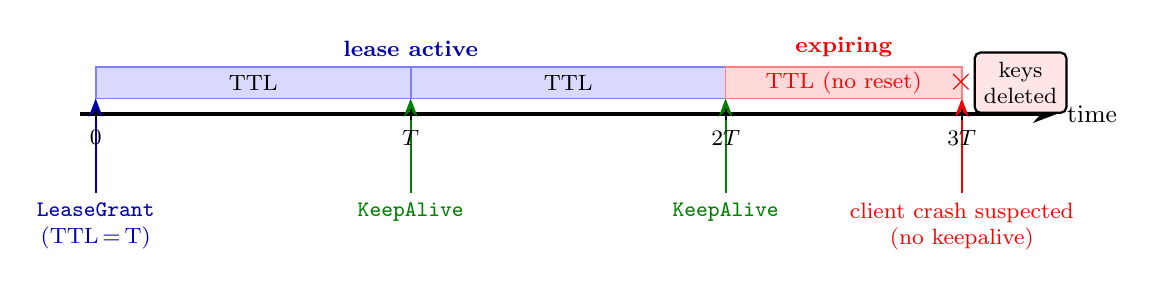
\begin{tikzpicture}[
    >=Stealth,
    thick,
    font=\small,
]

% ---- time axis ----
\draw[->, very thick] (-0.2, 0) -- (12.2, 0) node[right] {time};

% ---- active lease segments (green-ish while alive) ----
\fill[blue!15, draw=blue!50, line width=0.6pt] (0, 0.2) rectangle (4,   0.6);
\fill[blue!15, draw=blue!50, line width=0.6pt] (4, 0.2) rectangle (8,   0.6);
\fill[red!15,  draw=red!50,  line width=0.6pt] (8, 0.2) rectangle (11,  0.6);

\node[font=\footnotesize] at (2,   0.4) {TTL};
\node[font=\footnotesize] at (6,   0.4) {TTL};
\node[font=\footnotesize, red] at (9.5, 0.4) {TTL (no reset)};

% ---- events ----
% t=0: LeaseGrant
\draw[blue!70!black, ->]
  (0, -1.0) node[below, align=center, font=\footnotesize]
    {\texttt{LeaseGrant}\\(TTL\,=\,T)} -- (0, 0.2);

% t=4: first KeepAlive
\draw[green!50!black, ->]
  (4, -1.0) node[below, font=\footnotesize] {\texttt{KeepAlive}} -- (4, 0.2);

% t=8: second KeepAlive
\draw[green!50!black, ->]
  (8, -1.0) node[below, font=\footnotesize] {\texttt{KeepAlive}} -- (8, 0.2);

% t=11: expiry (no keepalive)
\draw[red, ->]
  (11, -1.0) node[below, align=center, font=\footnotesize, red]
    {client crash suspected\\(no keepalive)} -- (11, 0.2);
\node[font=\large\bfseries, red] at (11, 0.4) {$\times$};

% keys-deleted annotation
\node[draw, rounded corners=2pt, fill=red!10, font=\footnotesize,
      align=center, anchor=west] at (11.15, 0.4) {keys\\deleted};

% ---- tick marks and time labels ----
\foreach \t/\lbl in {0/0, 4/$T$, 8/$2T$, 11/$3T$} {
  \draw (\t, -0.07) -- (\t, 0.07);
  \node[below, font=\footnotesize] at (\t, -0.07) {\lbl};
}

% ---- state labels above bar ----
\node[above, font=\footnotesize\bfseries, blue!70!black] at (4, 0.6)
  {lease active};
\node[above, font=\footnotesize\bfseries, red] at (9.5, 0.6)
  {expiring};

\end{tikzpicture}


% ============================================================
% Figure 3: etcd 3-node cluster — write and read paths
%
% All writes go through the leader (Raft).
% Linearizable reads also go through the leader (or use the
% read-index protocol to confirm leader status without a full
% log round-trip).  Follower reads are opt-in and may be stale.
% ============================================================

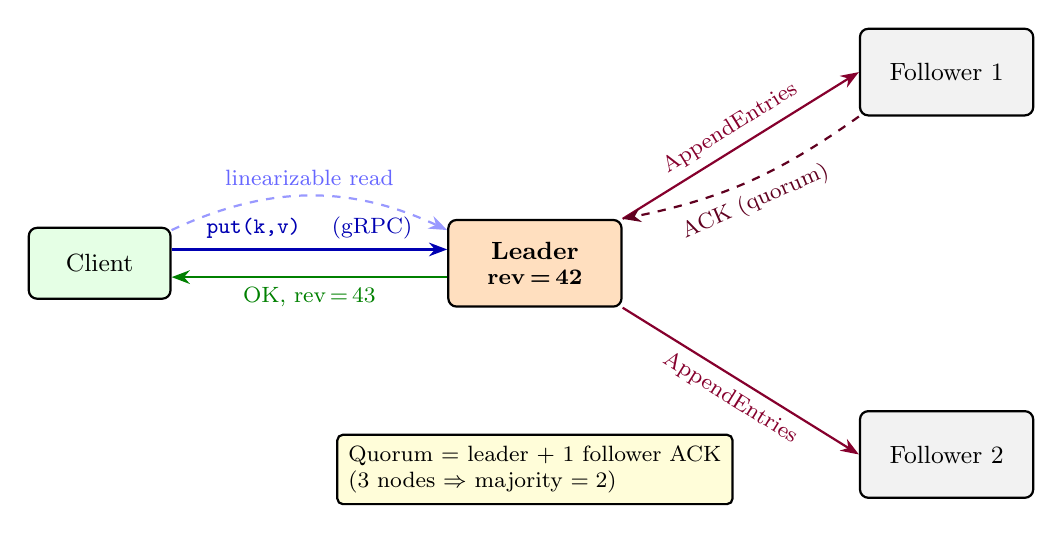
\begin{tikzpicture}[
    >=Stealth, thick, font=\small,
    server/.style={
      draw, rounded corners=3pt,
      minimum width=2.2cm, minimum height=1.1cm,
      align=center, fill=gray!10},
    leader/.style={
      draw, rounded corners=3pt,
      minimum width=2.2cm, minimum height=1.1cm,
      align=center, fill=orange!25, font=\bfseries\small},
    client/.style={
      draw, rounded corners=3pt,
      minimum width=1.8cm, minimum height=0.9cm,
      align=center, fill=green!10},
    note/.style={
      draw, rounded corners=2pt, fill=yellow!15,
      font=\footnotesize, align=left, inner sep=4pt},
]

\node[client]  (cl) {Client};
\node[leader,  right=3.5cm of cl]              (ld) {Leader\\[-2pt]{\footnotesize rev\,=\,42}};
\node[server,  above right=1.3cm and 3cm of ld] (f1) {Follower 1};
\node[server,  below right=1.3cm and 3cm of ld] (f2) {Follower 2};

% ---- write path: client -> leader -> ACK ----
\draw[->, blue!70!black]
  ([yshift= 5pt] cl.east) --
  node[above, font=\footnotesize] {\texttt{put(k,v)} \quad (gRPC)}
  ([yshift= 5pt] ld.west);

\draw[->, green!50!black]
  ([yshift=-5pt] ld.west) --
  node[below, font=\footnotesize] {OK, rev\,=\,43}
  ([yshift=-5pt] cl.east);

% ---- Raft replication: leader -> followers ----
\draw[->, purple!70!black]
  (ld.north east) --
  node[above, sloped, font=\footnotesize] {AppendEntries}
  (f1.west);

\draw[->, purple!70!black]
  (ld.south east) --
  node[below, sloped, font=\footnotesize] {AppendEntries}
  (f2.west);

% ---- quorum ACK: follower 1 -> leader ----
\draw[->, dashed, purple!50!black, bend left=12]
  (f1.south west) to
  node[below, sloped, font=\footnotesize] {ACK (quorum)}
  (ld.north east);

% ---- linearizable read path (dashed blue, same channel) ----
\draw[->, dashed, blue!40, bend left=25]
  ([yshift=12pt] cl.east) to
  node[above, font=\footnotesize, blue!60] {linearizable read}
  ([yshift=12pt] ld.west);

% ---- quorum callout ----
\node[note, below=1.6cm of ld] {
  Quorum = leader + 1 follower ACK\\
  (3 nodes $\Rightarrow$ majority $= 2$)
};

\end{tikzpicture}

\end{document}
